\documentclass{article}
\usepackage{float}
\usepackage[utf8]{inputenc}

\title{Projeto Multimédia - FlyBeat}
\author{André Batista \thanks{nº2012137523, amccbaptista@gmail.com} \and João L. Cardoso \thanks{nº2011151968, jaliborc@gmail.com} \and Rui F. Casaleiro \thanks{nº2012139327, rjfcasaleiro@gmail.com}}
\date{LEI - Meta 2}

\usepackage{natbib}
\usepackage{graphicx}

\begin{document}
\maketitle
\section{Resumo do Trabalho}
Neste trabalho iremos desenvolver um jogo de aviação inspirado em jogos como Audiosurf e GuitarHero. O jogador conduzirá um avião através de um túnel tridimensional evitando colidir com as paredes do mesmo. Haverá um número limite de colisões que um jogador pode fazer sem que isso resulte na perda do jogo.

O formato do túnel dependerá da análise de um ficheiro de música à escolha do utilizador, que servirá também como música de fundo para o jogo. Para esse efeito, analisaremos a melodia e a energia da mesma. Consideramos também a possibilidade da música poder criar turbulência na condução do avião em momentos-chave, e de o jogo poder ter efeitos sonoros dependendo do desempenho do jogador.

Um dos aspectos mais distintivos do jogo será possibilidade de controlar o avião utilizando os sensores de rotação de um smartphone Android. Como alternativa o avião poderá também ser controlado utilizando o teclado, mas iremos desenhar o jogo com o smartphone em mente.

Temos também o objectivo de ter, no menu inical, um registo do progresso do jogador em cada música - a percentagem da música à qual conseguiu "sobreviver" e com quantas falhas.

\section{Software Utilizado}
\subsection{Tecnologias}
\begin{itemize}
\item Away3D (Baseado em OpenGL)
\item Networking (Sockets TCP)
\item Android Sensors (Gyroscope - sensor de rotação)
\item Análise musical recorrendo a séries de Fourier
\end{itemize}

\subsection{Ferramentas}
\begin{itemize}
\item Adobe Flash Builer 4.7 (Desenvolvimento de código)
\item Flex 4.6 (Necessário para a library Away3D)
\item Android Developer Tools 22.3 (Desenvolvimento do controlo remoto)
\item Maya (Desenho de modelos 3D)
\item Adobe Fireworks CS5 (Planeamento de interfaces)
\item Prefab3D (Integração dos modelos produzidos na library Away3D)
\item Git (Desenvolvimento cooperativo)
\item Draw.IO (Desenho de esquemas auxiliares)
\end{itemize}

\section{Arquitectura}
\subsection{Diagramas de Navegação}
\begin{figure}[H]
\begin{center}
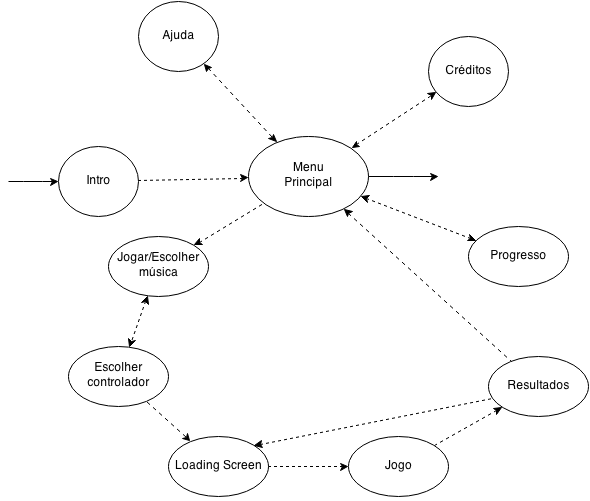
\includegraphics[scale=0.5]{Navigation.png}
\end{center}
\caption{Aplicação principal (jogo de computador)}
\end{figure}

\begin{figure}[H]
\begin{center}
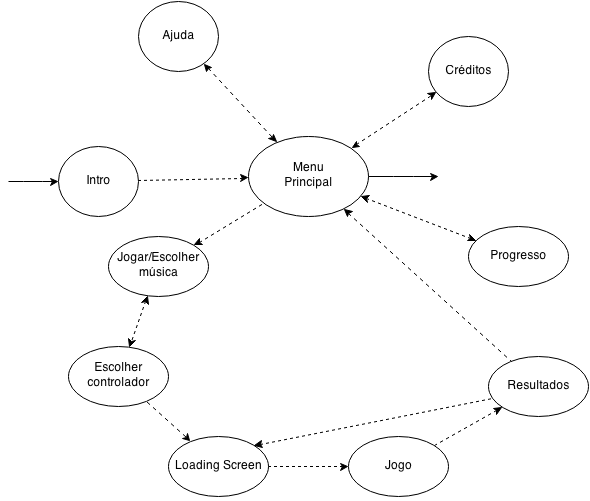
\includegraphics[scale=0.5]{Navigation.png}
\end{center}
\caption{Aplicação android (controlador)}
\end{figure}

\subsection{Diagramas de Classes Reduzidos}
\begin{figure}[H]
\begin{center}
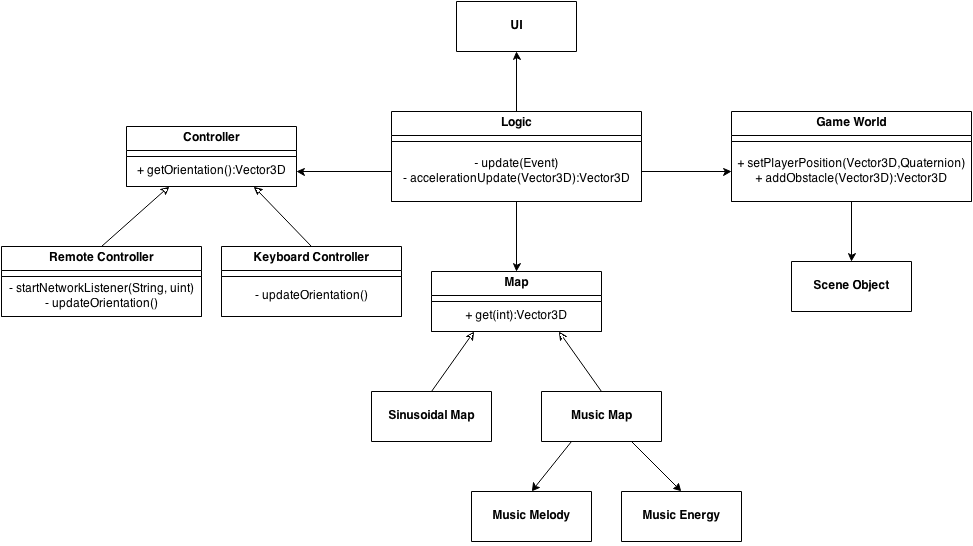
\includegraphics[scale=0.4]{Classes.png}
\end{center}
\caption{Aplicação principal (jogo de computador)}
\end{figure}

\begin{figure}[H]
\begin{center}
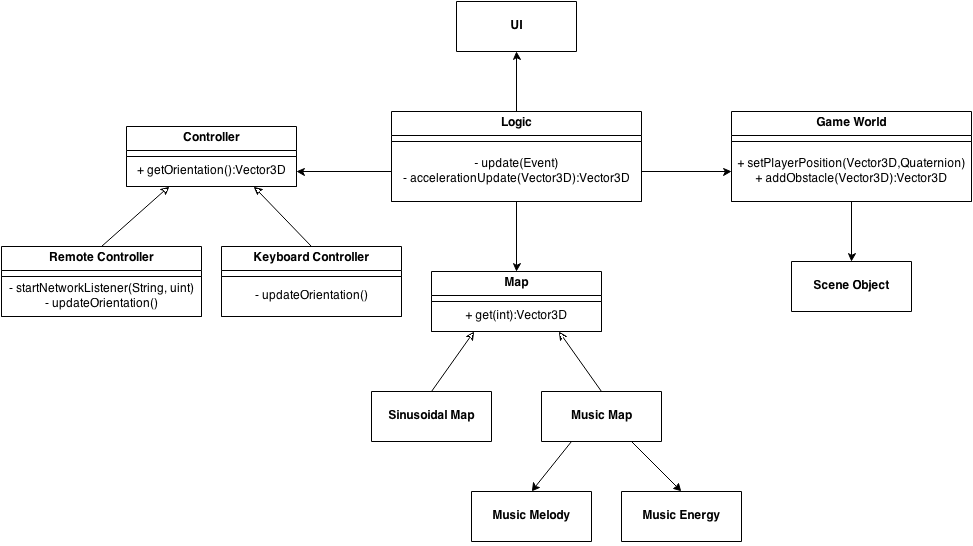
\includegraphics[scale=0.4]{Classes.png}
\end{center}
\caption{Aplicação android (controlador)}
\end{figure}

\section{Layout da Interface}
Tendo em conta o tipo de jogo que estamos a desenvolver e a sua estratégia de interação humano-computador - controlo através de posição física de um aparelho, poucos elementos do jogo serão representados através da user interface.

Assim sendo, o design da interface não só é secundário, como deverá ser feito em concordância com o gameplay final. A maioria da user interface será consituída por menus de controlo a serem usados antes e após cada jogo. Portanto, decidimos realizar o design da interface numa fase mais tardia do projeto.

No entanto, apresentamos algumas imagens representativas de um possível layout dos menus iniciais.

\begin{figure}[H]
\fbox{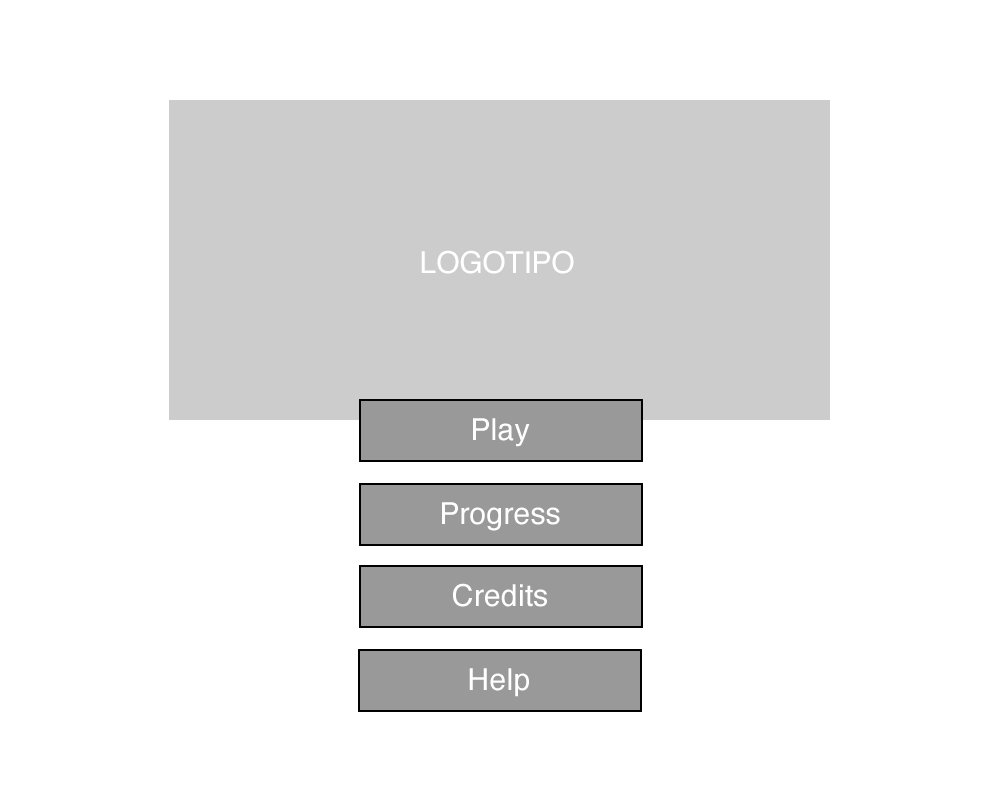
\includegraphics[scale=0.15]{MainMenu.png}}
\fbox{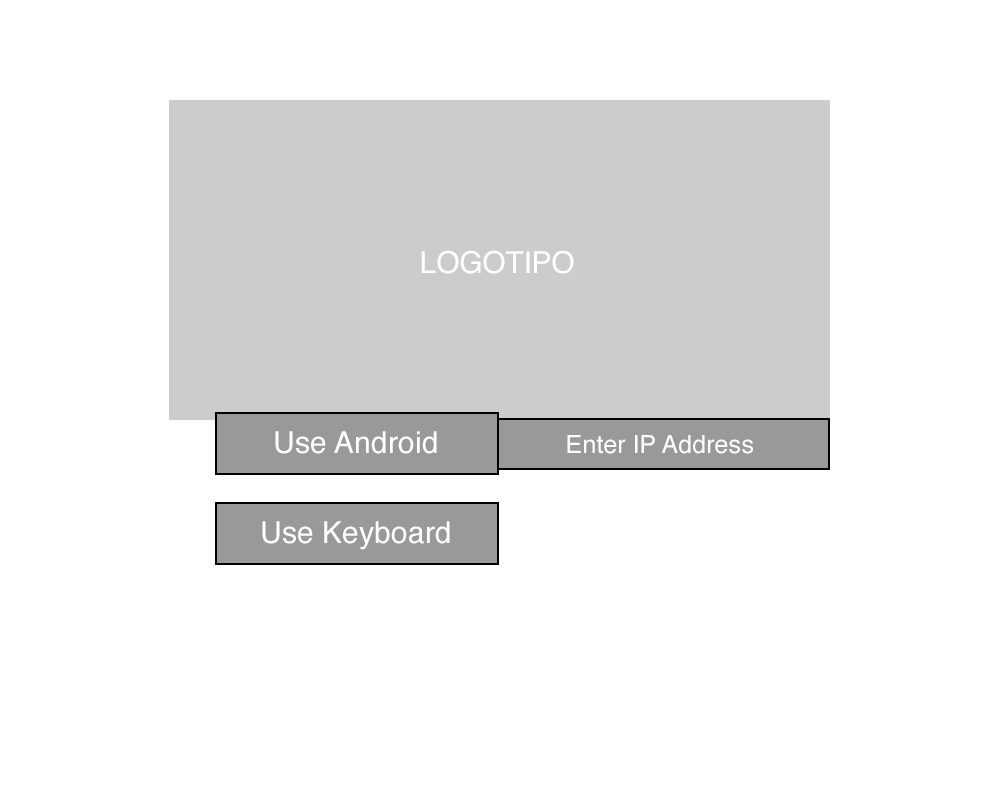
\includegraphics[scale=0.15]{ControllerSelect.png}}
\caption{Esquerda: menu principal. Direita: escolha de controlador (em princípio, será necessário introduzir o endereço IP do android mas, idealmente, faremos deteção automática de devices)}
\end{figure}

\section{Preview de Gameplay}
Actualmente, já conlcuímos grande maioria da framework necessária para terminar o jogo. Por isso dispomos já de um primeiro demo do jogo funcional com um mapa gerado segundo funções sinusoidais.

Todo o desenvolvimento relativo a networking, game logic e 3D está pronto, faltando assim realizar a análise musical, cyclic development e testing de gameplay e, finalmente, design de um look final para o jogo. Como já expresso anteriormente, a user interface e logótipo serão desenvolvidos após estes passos.

Para um preview do estado atual do jogo, por favor veja este teaser: 

\section{Diagrama de Gant}

\end{document}